\section{Violent Deaths. Examples.}

The opposition of Sun and Moon is not always bad. Only if an approaching malefic beholds the phase\footnote{Most likely the syzygy, New or Full Moon, before birth.} or if the malefic casts its rays while it has some relationship with the luminaries does the opposition become bad. Consequently, even the all-fortunate nativities do not remain lucky to the end; at \textbf{/124K/} some place the houserulership of the star \textbf{/118P/} becomes badly situated or reversed and causes ill fortune.

Petosiris\mn{Petosiris} seems to have defined the place perfectly, even though he spoke in mystic riddles: \begin{quote}The
beginning, the end, the controller, and the measurement standard of the whole is the houseruling star of
each nativity: it makes clear what kind of person the native will be, what kind of basis his livelihood will have, what his character will be, what sort of body <=health and appearance> he will have, and all the things that will accompany him in life. Without this star nothing, neither occupation nor rank, will come to anyone.\end{quote}

But, how is it possible for a nativity to succeed in everything or, on the other hand, to fail in everything, depending just on the houserulership of just one star? On the contrary, generally one star is found to be ruler of the basis\mn{Basis} of the nativity (i.e. noble, average, base-born) from its beginning (or that one star activates the influences of the rest). Another star is the ruler of the remaining factors. We see some men fortunate in their livelihood and public standing, adorned with all magnificence, with the apparent houseruler configured appropriately. <We see> these same men, however, to be unfortunate in the wives
and children, becoming outrageous and disgusting, polluting their livelihood, and becoming public scandals as if they were unworthy of their excellent beginnings. Some are even ruined later or die violently. Therefore the native is not fortunate in everything nor does everything happen as the consequence of <one> houseruler. Another afflicted houseruler blackens reputations by bringing many crises. We also note that other men have gone from a low and ignoble station to an unsurpassed and unhoped-for condition. We note others who are fortunate in their wives and children, but needy in their livelihood. Still others are prosperous in possessions, but of low rank and sickly. Others are long-lived, but toil-worn and crippled. Some are rich but short-lived or consumptive, and hence unable to profit from their riches. So we say: one star is the Life-giver, another is the ruler of property and of death.

But, someone will say, if the houseruler is unfavorably situated, the native will be short-lived. For that very reason, since it is unfavorably situated, it is of no use for <the houseruler> to grant a prosperous livelihood, \textbf{/125K/} nor would it be appropriate for the houseruler to make a subjugated and base-born native illustrious and distinguished later in life. Nor will a well-configured star cause a high-born native, one never \textbf{/119P/} entangled in evildoing, to be condemned and to die violently. Instead, the unfavorably situated star creates the lesser man, but the ruler of rank and livelihood, found at an angle and receiving the chronocratorship, renders the man illustrious. If so, then this star which makes the man fortunate, if found at an angle or in operative places, keeps him fortunate during its own chronocratorship. But when the star comes to have another star which causes disease, infirmity, or some other critical affliction in superior aspect or in opposition, then it will yield and its influence will weaken. 

Many other noteworthy things happen in the life of man, things which come about not through the activity or operation of one houseruler, but through the activity of many. If anyone researches thoroughly the Places and the houserulers, he will determine quite easily the area in which the nativity is fortunate and the area in which it is unfortunate. Whenever any star that has a relationship with the nativity (i.e. one that controls livelihood, life, injury, disease, occupation, or any of the other areas of concern) is afflicted in one respect, in that respect it will harm the nativity. Indeed, we
find that the Compiler does not use <just> one influential houseruler. He says: \begin{quote}One controls occupations, one the possession of years, one stability and change, one decline; \end{quote}
or again:
\begin{quote}Observing the positions of the sun and moon at conjunction and their separations after full moon, with
respect to the angles and the signs following them, on which the whole <forecast> depends;\end{quote}
or again:
\begin{quote}When starting to cast a horoscope, one must examine the Descendant, the sign preceding the Descendant,
and the sign just following the Descendant, because in these places is found the fated outcome.\end{quote}

He says many other similar things. So it is necessary to consider one place for occupation and rank, another for life, another for injury, disease, and death. Not everything will depend on one houseruler. We act rationally when we make our forecasts after considering many influences. Later in our treatise we will clarify these points, \textbf{/126K/} particularly in <the section on> the distribution of the chronocratorships. Now we will press on to consider violent deaths. 

When the ruler of the new or full moon at the nativity is turned away from its sign or is unfavorably situated, with a malefic in aspect, it indicates violent death. In the same way, if \Mercury\xspace is in opposition to the full moon and has malefics in aspect, it brings a bad cause of death. 

If Saturn, Mars, or Mercury are located in the sign <of the \Moon> on the fortieth day, \textbf{/120P/} they indicate violent death. Likewise malefics in the Descendant or
in the sign preceding the Descendant bring violent deaths or the onset of diseases and miserable deaths.

The VIII Place from the Ascendant has the same influence on the cause of death; so does the 8th Place from the Lot of Fortune. It is necessary to examine the Lot and its ruler to see in which signs they are located, because the cause of death will be foretold by them: the Moon (which is Fortune), when in conjunction with the \Sun\xspace in \Aries, suffers an eclipse or loss of light in the eighth sign, Scorpio. Therefore Scorpio is called its depression.

% -- Signs --------------------------------------------------
\subsection{\textit{[Indications from Signs]}}
We will give a brief tour of each sign in order to make what is said here easily understandable:

Aries \mn{\Aries} is destroyed by Scorpio. Since they are both domiciles of Mars, Mars is a destroyer of itself. Therefore <Aries> causes suicides, those who throw themselves from heights, and those ready for death;
accomplices in crime, bandits, and murderers (i.e. those who bring a cause of death on themselves), plus those perishing from animal attacks, from fires, or from collapsing buildings. <It also causes men to die> from animals, bleeding, or attacks.

Taurus \mn{\Taurus} is destroyed by Sagittarius, i.e. Venus is destroyed by Jupiter. Men born under this configuration die peacefully from luxurious living, from stuffing themselves with food, wine, or sex, or from strokes
while asleep or while relaxing. No distressing cause of death will appear, unless some malefic in conjunction or in aspect introduces and indicates a cause of death appropriate to its nature.

Gemini \mn{\Gemini} is destroyed by Capricorn, i.e. Mercury by Saturn. Some men die violently troubled by black bile, are attacked by painful cramps or are harmed in damp places by beasts or by crawling things. Some are condemned to death, \textbf{/127K/} imprisoned, or suffocated. Some are attacked by bandits or the enemy. Some are poisoned—because of the wet quality <of the sign>.

Cancer \mn{\Cancer} is destroyed by Aquarius, i.e. the Moon by Saturn. Men perish through dampness or internal complaints, from pains of the spleen and stomach, or from vomiting fluids. They die at sea, on rivers, from chills, from attacks of beasts and crawling things. They perish from elephantiasis, jaundice, lunacy, poisoning, long imprisonment, and other chronic fevers. Women die from pains of the breasts, cancer, infirmities of the genitals or womb, from suffocation, or from abortions.

Leo \mn{\Leo} is destroyed by Pisces, i.e. the Sun by Jupiter. As a result men die from heart attacks \textbf{/121P/} and from complaints of the liver. They are at risk in wet places or from moist complaints, falls, the ague, accidents in the baths, and the treachery of women.

Virgo \mn{\Virgo} is destroyed by Aries, i.e. Mercury by Mars. They die from treachery and crime. They are attacked by the enemy or by bandits. They perish from burns, collapsing buildings, blindness, imprisonment, the wrath of noblemen, or from captivity, falls from animals or high places, the crushing of limbs, or animal attacks. Females die from collapsed uterus, abortions, hemorrhages, or consumption.

Libra is destroyed by Taurus, i.e. Venus by itself. Therefore men become suicides through poisoned drinks, through snakebite, through self-starvation. They die from excessive intercourse, excision of the uvula, drowning, or they become mutilated, blind, or paralyzed. They are attacked by females or fall from high places or animals.

Scorpio \mn{\Scorpio} is destroyed by Gemini, i.e. Mars by Mercury. They die by knife cuts to the genitals or the rump, or from strangury, festering sores, choking, crawling things, violence, war, attacks by bandits, assaults of pirates, or because of officials, and by fire, impaling, attacks of beasts and crawling things.

Sagittarius \mn{\Sagittarius} is destroyed by Cancer, i.e. Jupiter by the Moon. They die from disorders of the spleen, liver, stomach, from vomiting fluids or blood, falls from animals, attacks of ravenous beasts, collapsing buildings, shipwreck, wet places. They die from lunacy, blindness, feebleness. 

Capricorn \mn{\Capricorn} is destroyed by Leo, i.e. Saturn by the Sun. They die from heart attacks and fractures and from accidents in the baths or from burns, through the wrath of kings and noblemen, or by impaling, injuries from beasts and animals, or falls from high places.

Aquarius \mn{\Aquarius} is destroyed by Virgo, i.e. Saturn by ercury. They die \textbf{/128K/} from wasting of the vitals, dropsy, elephantiasis, jaundice, fever, sword slashes, dysentery, and from the treachery of women.

Pisces \mn{\Pisces} is destroyed by Libra, i.e. Jupiter by Venus. <They die> from moist complaints, poisoning, painful fluxes or cramps, complaints of the genitals or liver, sciatica, attacks of beasts and crawling things.

% -- Examples -----------------------------------------------
\subsection{\textit{Examples}}
So much for the subject of violent death. In addition it will be necessary to take into account the influence of each sign on injuries and diseases so as to \textbf{/122P/} make the type of death obvious. Each star in conjunction or aspect will have the effect of adding its influence to the cause of death according to the star’s nature. It is necessary to examine how the Places and their rulers are situated and whom they have in
aspect (viz. related or unrelated stars), and thus make your determination. Malefics in conjunction with the Places or in aspect with the houserulers bring violent death. Benefics indicate the cause to be distress, injury, disease, or an attack of fever. 

For example: \Gemini\, is destroyed by \Capricorn\, and \Aquarius\, by \Virgo, i.e. \Mercury\, by \Saturn\, and \Saturn\, by \Mercury. Now if these stars have the relationship of opposition or square in a nativity, they cause men to have short lives or a wretched death, since the Lifegiver\footnote{The ruler of the Ascendant.} is in opposition to the ruler of Death\footnote{The ruler of the 8th place.}. If they have no relationship, but simply \mn{beholding} behold each other without being in their own domiciles, they bring setbacks, trials, exile, and other temporary misfortunes\footnote{Think Valens is saying that if the two planets are in aspect but do not rule the 1st and 8th (are not related to life and death) they bring on difficulties but not necessarily death.  Note that if they were in their own domiciles they would conceivably still have a 1st-8th relationship that could be activated during a profection.}. (Consider the arrangement of \Mars\, and \Mercury\, as having the same effects.) The Old Astrologer wants them to be in opposition when he says: \begin{quote}Let every opposing configuration (=rising and setting) of any star or of the Sun and the Moon cause the native to be subject to the legal process.\end{quote}

But I declare that crises concerning rank, livelihood, and death will occur, if the stars have a relationship involving destruction or some other houseruling function.
\newpage
% -- Chart 1 ---------------------------------------------31-
\subsubsection{\textit{[Chart 31: Drowning ]}}
Examples: \Sun, \Mars, \Venus\xspace in \Cancer, \Saturn, \Mercury\xspace in \Leo, \Jupiter\xspace in \Aquarius, \Moon\xspace in \Pisces, Ascendant in \Scorpio, the Lot of Fortune in \Leo, the <8th> Place of Death\footnote{\Pisces\xspace is the 8th from the Lot of Fortune.} in \Pisces\footnote{\textit{Greek Horoscopes} dates the chart (L123) to approximately July 2, 123 AD (p.122)}.

\clearpage
\begin{wrapfigure}[15]{R}{7cm}
\centering
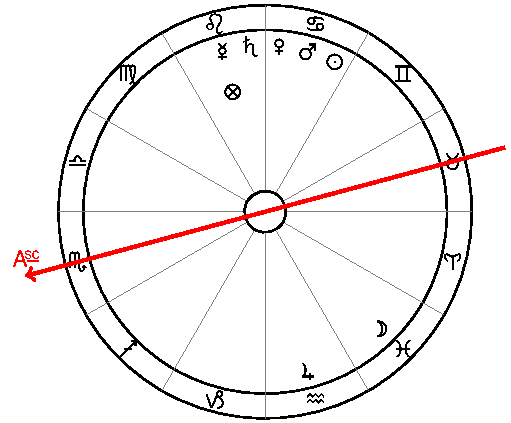
\includegraphics[width=0.68\textwidth]{charts/2_41_1}
\caption{Chart 31 [II.41.1, GH L123]}
\label{fig:chart31}
\end{wrapfigure} 

The \Moon\xspace was in this Place\textsl{[\Pisces]}, and \Saturn\xspace was in conjunction with the Lot of Fortune. The ruler <of \Leo>, the \Sun, was with \Mars\xspace in \Cancer, a wet sign\footnote{Robert Hand points out that \Mercury\, and \Saturn\, are ``mutual destroyers'' (\Virgo, ruled by \Mercury, is the 8th place from \Capricorn, ruled by \Saturn\, who, even though in sect, is also in his detriment and so possibly more malefic). Both are conjunct the Lot of Fortune. As well, the \Sun, the ruler of the Lot, is conjunct \Mars, who is the contrary to sect malefic and in his fall in \Cancer\, (VRS3 p17).}. 

This person died in the bath, drowned in the water. \Mars\xspace was in opposition to the full moon <\Capricorn>, and \Saturn, the ruler <of the full moon>, was turned away. Therefore he died violently.\textbf{/129K/}
\newpage
% -- Chart 2 ---------------------------------------------32-
\subsubsection{\textit{[Chart 32: Beheaded]}}
Another example: \Sun, \Mercury, \Venus\xspace in \Pisces, \Saturn\xspace in \Virgo, \Jupiter\xspace in \Aries, \Mars\xspace in \Taurus, \Moon\xspace in \Sagittarius, Ascendant in \Leo, the Lot of Fortune in \Taurus
\footnote{\textit{Greek Horoscopes} dates the chart (L97) to approximately February 23, 97 AD (p.98)}.  

\clearpage
\begin{wrapfigure}[15]{R}{7cm}
\centering
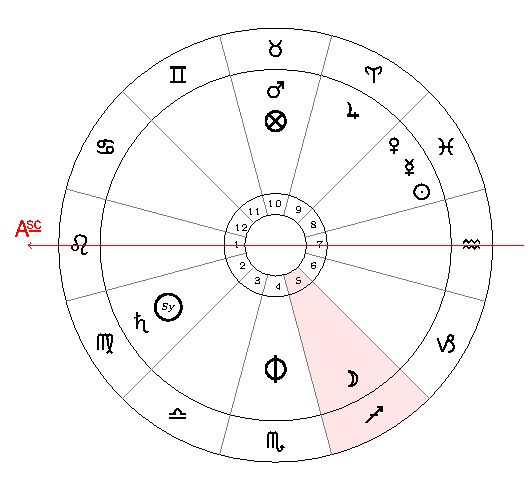
\includegraphics[width=0.68\textwidth]{charts/2_41_2}
\caption{Chart 32 [II.41.2, GH L97]}
\label{fig:chart32}
\end{wrapfigure} 

\noindent \Mars\xspace was located so that it ruled Daimon <\Scorpio> and was in opposition to it. 

The <8th> Place of Death\footnote{From Fortune.} was in \Sagittarius, and the \Moon\xspace was there and had \Saturn\xspace in superior aspect in the sign of the full moon <\Virgo>. 

Likewise \Mercury, the ruler of the full moon, was in opposition <to \Virgo\xspace and Saturn>. 

The native was beheaded\footnote{Robert Hand says \Taurus, where Fortune is, emphasizes the throat. Detrimented \Mars, the contrary to sect malefic, ruling and opposed to Spirit, ``indicates danger of injury'' while \Saturn\, overcoming the \Moon\, in the 8th from Fortune ``adds to the fatality of the combination'' (VRS3 18).

Note as well that \Mars\, acts by cutting and \Jupiter, ruler of the 8th from Fortune, is averse to \Mars\, and his own house, \Pisces, on the radix 8th and so indicates a violent death.}.\textbf{/123P/} 
\newpage
% -- Chart 3 ---------------------------------------------33-
\subsubsection{\textit{[Chart 33: Beheaded]}}
Another example: \Sun\xspace in \Cancer, \Moon\xspace in \Pisces, \Saturn, \Mars, \Mercury\xspace in \Gemini, \Jupiter\xspace in \Capricorn, \Venus\xspace in \Leo, Ascendant in \Libra, the Lot of Fortune in \Gemini
\footnote{\textit{Greek Horoscopes} dates the chart (L87) to approximately July 9, 87 AD (p.95)}.

\clearpage
\begin{wrapfigure}[15]{R}{7cm}
\centering
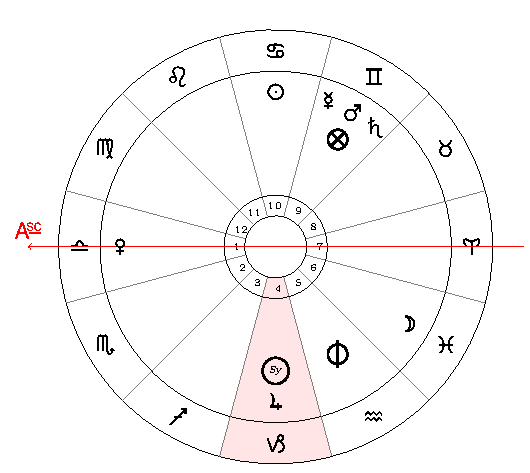
\includegraphics[width=0.68\textwidth]{charts/2_41_3}
\caption{Chart 33 [II.41.3, GH L87]}
\label{fig:chart33}
\end{wrapfigure} 

In this sign \textsl{[\Gemini]} \Saturn, \Mercury, and \Mars\xspace attended each other, being destroyers of each other, and they were in aspect with the \Moon\xspace <\Square>. 

Likewise the ruler <\Saturn> of the full moon <\Capricorn> was turned away, and \Jupiter\xspace in the <8th> Place of Death\footnote{\Jupiter\, is in \Capricorn, the 8th from Fortune.} and in opposition to the \Sun\xspace was not able to help. The native was beheaded\footnote{Robert Hand points out that \Mercury, \Mars, and \Saturn\, are all mutual destroyers posited with Fortune and averse to \Jupiter\, in the 8th from Fortune, who can offer no help (VRS3 19). Also note that \Jupiter\, rules the \Moon\, (the body) in \Pisces\, in the radix 6th of injury. The throat is possibly being shown by \Taurus\, on the radix 8th.}.
\newpage
% -- Chart 4 ---------------------------------------------34-
\subsubsection{\textit{[Chart 34: Beheaded]}}
Another example: \Sun, \Mercury, \Mars, \Jupiter, \Venus\xspace in \Capricorn, \Moon\xspace in \Aquarius, \Saturn\xspace in \Taurus, Ascendant in \Aries
\footnote{\textit{Greek Horoscopes} dates the chart (L86) to approximately December 27, 86 AD (p.94). Fortune and Spirit added for reference.}.

\clearpage
\begin{wrapfigure}[1]{R}{7cm}
\centering
\vspace{-20pt}
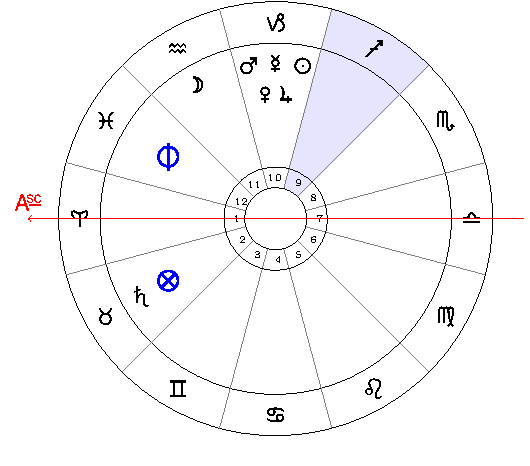
\includegraphics[width=0.68\textwidth]{charts/2_41_4}
\caption{Chart 34 [II.41.4, GH L86]}
\label{fig:chart34}
\end{wrapfigure} 

The native was beheaded\footnote{Robert Hand, referring to the loaded 10th house, puts the beheading down to the multiplicity of ``destroyer-destroyer pairings'' as  \Jupiter\, and \Venus\, destroy each other, \Jupiter\, conjunct the \Sun\, destroys the \Sun, and \Mercury\, and \Mars\, destroy each other (VRS3 p20).
  
If Fortune (from the \Sun\, to the \Moon projected from the Asc) is in \Taurus\, it is with \Saturn, ruler of all those 10th house destroyer-pairings and overcome by them and, the 8th from Fortune, the Place of Death, would be in \Sagittarius, ruled by a \Jupiter\, who is also with all the destroyer pairs and is in aversion to his own place, indicating a violent end.}.
\newpage
% -- Chart 5 ---------------------------------------------35-
\subsubsection{\textit{[Chart 35: Roasted in his Bath]}}
Another example: \Sun, \Venus\xspace in \Aquarius, \Moon\xspace in \Gemini, \Saturn\xspace in \Scorpio, \Jupiter\xspace in \Pisces, \Mars\xspace in \Cancer, \Mercury, Ascendant in \Capricorn, the Lot of Fortune in \Virgo, the <8th> Place of Death in \Aries
\footnote{\textit{Greek Horoscopes} dates the chart (L101) to approximately January 28, 101 AD (p.99)}.

\clearpage
\begin{wrapfigure}[12]{R}{7cm}
\centering
\vspace{-20pt}
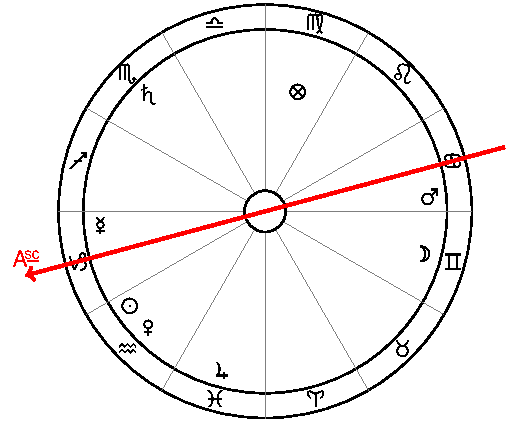
\includegraphics[width=0.68\textwidth]{charts/2_41_5}
\caption{Chart 35 [II.41.5, GH L101]}
\label{fig:chart35}
\end{wrapfigure}

The rulers <\Mercury\, \Mars> of these places were in opposition to each other and in wet signs; furthermore \Mars\xspace was in the Descendant. 

The native was roasted while relaxing in the bath\footnote{Robert Hand notes that Valens and other early astrologers considered \Capricorn\, a \textsl{wet} sign and that the main point appears to be the opposition between the ruler of the Lot of Fortune (\Mercury) and the 8th from Fortune (\Mars) being destroyers of each other (VRS3 p20).  Also of interest, again, is the aversion of benefics, with the sect benefic (\Venus) averse to Fortune and the contrary to sect benefic (\Jupiter) averse to the 8th from Fortune, with aversion indicating a violent death.}. 
\newpage
% -- Chart 6 ---------------------------------------------36-
\subsubsection{\textit{[Chart 36: Burnt Alive ]}}
Another example: \Sun, \Venus\xspace in \Capricorn, \Moon\xspace in \Cancer, \Saturn, \Mercury\xspace in \Sagittarius, \Jupiter\xspace in \Taurus, \Mars\xspace in \Leo, Ascendant in \Aquarius, the Lot of Fortune in \Leo
\footnote{\textit{Greek Horoscopes} dates the chart (L103) to approximately January 10, 103 AD (p.101-2)}.

\clearpage
\begin{wrapfigure}[12]{R}{7cm}
\centering
\vspace{-20pt}
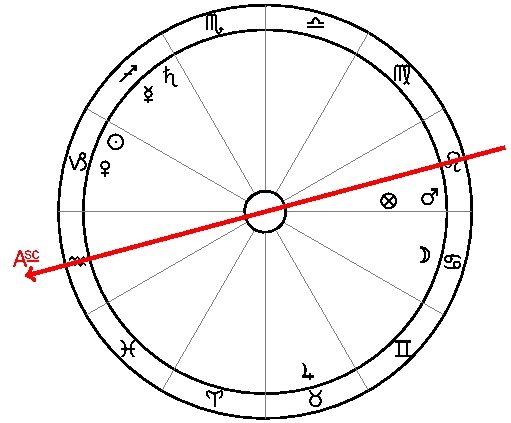
\includegraphics[width=0.68\textwidth]{charts/2_41_6}
\caption{Chart 36 [II.41.6, GH L103]}
\label{fig:chart36}
\end{wrapfigure}

\noindent \Mars\xspace was in \Leo, a fiery and solar sign, in opposition to the Ascendant. 

Saturn and \Mercury\xspace were in superior aspect to the <8th> Place of Death <\Pisces>. 

The native was burned alive\footnote{Robert Hand says the main point appears to be \Mars\, \Conjunction\, \Fortune\, in opposition to the Ascendant and the overcoming square of the mutual destroyers, \Mercury\, and \Saturn\, to the 8th from Fortune (VRS3 21); however, think we  also need to consider that \Mercury\, rules the radix 8th of death  and \Saturn\, the Ascendant, with both posited in \Sagittarius\, whose ruler, \Jupiter, is averse and also ruler of the 8th from Fortune  and so is of no help in averting the death.}.
\newpage
% -- Chart 7 ---------------------------------------------37-
\subsubsection{\textit{[Chart 37: Thrown to the Lions]}}
Another example: \Sun\xspace in \Capricorn, \Moon\xspace in \Libra, \Saturn\xspace in \Taurus, \Jupiter\xspace in \Gemini, \Mars, Ascendant in \Cancer, \Venus\xspace in \Aquarius, \Mercury\xspace in \Sagittarius, the Lot of Fortune in \Libra
\footnote{\textit{Greek Horoscopes} dates the chart (L115) to approximately December 26, 115 AD (p.112)}. 

\clearpage
\begin{wrapfigure}[13]{R}{7cm}
\centering
\vspace{-20pt}
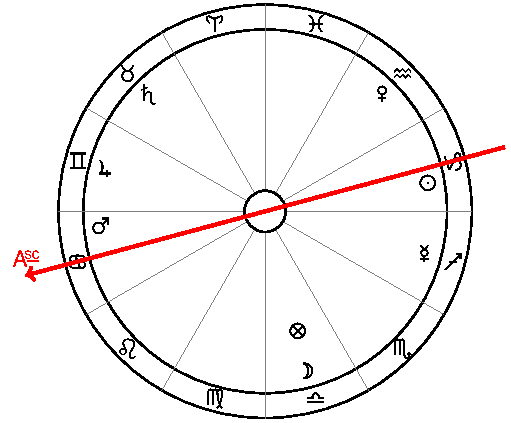
\includegraphics[width=0.68\textwidth]{charts/2_41_7}
\caption{Chart 37 [II.41.7, GH L115]}
\label{fig:chart37}
\end{wrapfigure}

The \Moon\xspace was in \Libra\xspace and was in inferior aspect to \Mars, which was in opposition to the \Sun. 

The <8th> Place of Death was in \Taurus, and \Saturn\xspace was there. 

The native was thrown to the lions\footnote{Robert Hand notes that both the Lot of Fortune and the 8th from Fortune are ``afflicted by malefics'' with \Mars\, and the \Sun\, square Fortune and \Saturn\, in the 8th from Fortune. As well, \Venus\, acts to destroy itself, ruling both Fortune and the 8th from Fortune and posited in the radix 8th square \Saturn\, in the Fortune 8th (VRS3 22). 

We should also note that the \Moon, ruling the Ascendant, is destroyed by \Saturn, ruling the radix 8th with both also disposited by \Venus; in fact, \Venus\, and \Saturn\, are in mutal reception by domicile, they can fully act for each other and both are determined to the native's end.}. \textbf{/130K/} 
\newpage
% -- Chart 8 ---------------------------------------------38-
\subsubsection{\textit{[Chart 38: Poisoned]}}
Another example: \Sun, \Moon, \Mercury\xspace in \Gemini, \Saturn\xspace in \Leo, \Jupiter\xspace in \Pisces, \Mars\xspace in \Cancer, \Venus\xspace in \Taurus, Ascendant in \Capricorn. The Lots were also in \Capricorn
\footnote{\textit{Greek Horoscopes} dates the chart (L65) to approximately May 24, 65 AD (p.84)}. 
 
\clearpage
\begin{wrapfigure}[10]{R}{7cm}
\centering
\vspace{-20pt}
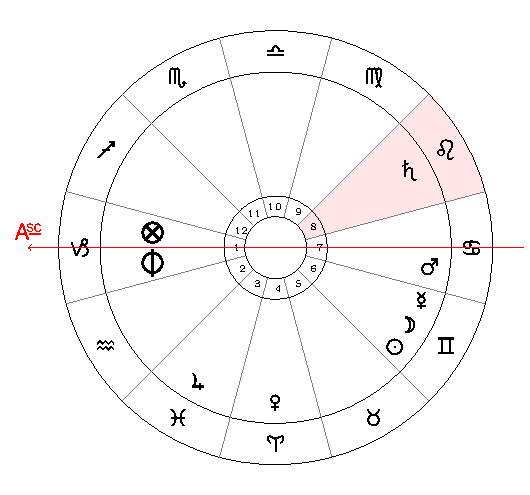
\includegraphics[width=0.68\textwidth]{charts/2_41_8}
\caption{Chart 38 [II.41.8, GH L65]}
\label{fig:chart38}
\end{wrapfigure} 
 
The ruler <of the Lots>, \Saturn, was in the <8th> Place of Death <\Leo> and was beheld by \Venus. \

Mars was in opposition to the Ascendant. 

The native died by poison\footnote{Robert Hand  says ``Here again we have the Lot of Fortune afflicted by \Mars\, in the 7th house, \Venus\, in square to the Lot, and \Saturn\, in the eighth house from both the \textsl{H\={o}roskopos} and the Lot. The trine from \Venus\, to \Saturn\, is the indicator of poison. Also recall tha \Venus\, destroys itself because \Taurus\, is the eighth from \Libra\, (VRS23). Also of note is that once more, \Jupiter\, is averse, this time to \Saturn\, and \Venus\, so it cannot intercede.}.
\newpage
% -- Chart 9 ---------------------------------------------39-
\subsubsection{\textit{[Chart 39: Drowned]}}
Another example: \Sun, \Mercury, Ascendant in \Taurus, \Moon\xspace in \Pisces, \Saturn\xspace in \Gemini, \Jupiter\xspace in \Aquarius, \Mars\xspace in \Virgo, \Venus\xspace in \Aries, the Lot of Fortune in \Pisces
\footnote{\textit{Greek Horoscopes} dates the chart (L88) to approximately May 5, 88 AD (p.95)}.   

\clearpage
\begin{wrapfigure}[12]{R}{7cm}
\centering
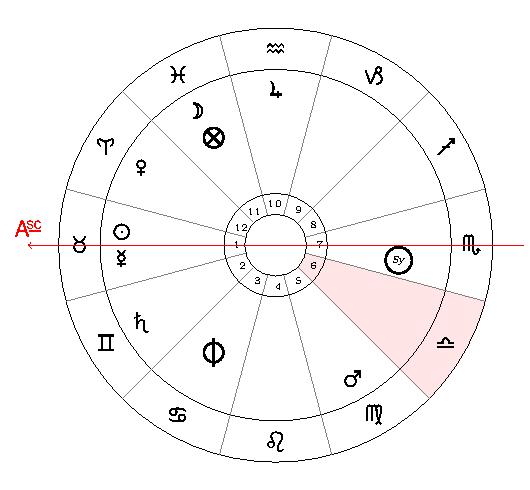
\includegraphics[width=0.68\textwidth]{charts/2_41_9}
\caption{Chart 39 [II.41.9, GH L88]}
\label{fig:chart39}
\end{wrapfigure} 

The \Moon\xspace was in \Pisces\xspace beheld by \Saturn\xspace and \Mars. 

The ruler <\Moon> of Daimon <\Cancer> and the ruler <\Mars> of the full moon <\Scorpio> were in opposition. 

The native drowned in bilge water\footnote{The \Moon, ruler of Daimon, Fortune, Daimon, and the syzygy were all in water signs, trine each other with both benfics (\Venus\, and \Jupiter) averse to the \Moon\, and Fortune while \Mars\, opposed and was being overcome by the square of \Saturn.}. \textbf{/124P/} 
\newpage
% -- Chart 10 --------------------------------------------40-
\subsubsection{\textit{[Chart 40: Hung Himself]}}
Another example: \Sun\xspace in \Leo, \Moon, \Mercury\xspace in \Virgo, \Saturn\xspace in \Gemini, \Jupiter\xspace in \Aries, \Mars, Ascendant, \Venus\xspace in \Cancer, the Lot of Fortune in \Gemini
\footnote{\textit{Greek Horoscopes} dates the chart (L89) to approximately July 29, 89 AD (p.96)}. 

\clearpage
\begin{wrapfigure}[14]{R}{7cm}
\centering
\vspace{-20pt}
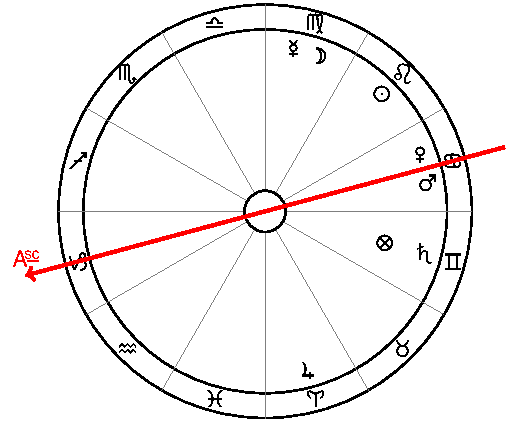
\includegraphics[width=0.68\textwidth]{charts/2_41_10}
\caption{Chart 40 [II.41.10, GH L89]}
\label{fig:chart40}
\end{wrapfigure} 

\noindent\Saturn, the ruler <of the 8th Place> of Death was in \Gemini\xspace and in superior aspect to \Mercury, the ruler of the Lot of Fortune, and to the \Moon. Furthermore \Mars\xspace was in opposition to the <8th> Place of Death <\Capricorn>. 

The native hanged himself\footnote{\Saturn, the ruler of the 8th from Fortune, is conjunct Fortune and averse to its own domicile (\Capricorn) while \Mars\, opposes the 8th from Fortune and is averse to Fortune and \Saturn. \Venus\, is with \Mars\, and averse to Fortune and the 8th from Fortune so of no help. \Jupiter\, is not averse but he is in \Mars's domicile (\Aries) and in superior (overcoming) square to \Mars\, as well as being square the 8th from Fortune, so also of no help.}.
\newpage
% -- Chart 11 ---------------------------------------------41-
\subsubsection{\textit{[Chart 41: Thrown to the Lions]}}
Another example: \Sun, \Mercury\xspace in \Aries, \Moon, \Venus\xspace in \Pisces, \Saturn\xspace in \Cancer, \Jupiter, \Mars\xspace in \Taurus, Ascendant in \Scorpio, the Lot of Fortune in \Sagittarius
\footnote{\textit{Greek Horoscopes} dates the chart (L91) to approximately April 4, 91 AD (p.96)}. 

\clearpage
\begin{wrapfigure}[14]{R}{7cm}
\centering
\vspace{-20pt}
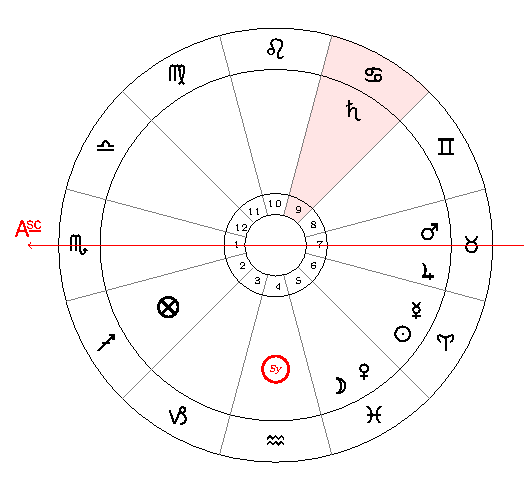
\includegraphics[width=0.68\textwidth]{charts/2_41_11}
\caption{Chart 41 [II.41.11, GH L91]}
\label{fig:chart41}
\end{wrapfigure} 

The ruler <\Jupiter, of the Lot of Fortune> was in the Descendant with \Mars. 

The <8th> Place of Death was in \Cancer. \Saturn, the ruler of the full moon<?>, was turned away\footnote{Assuming the syzygy was in \Aquarius\, which is ruled by \Saturn\, and averse to \Cancer. \textsl{Greek Horoscopes} suggests \Libra\, which \Saturn\, rules by exaltation but that is not ``turned away'' from \Cancer.} and \Mars\xspace was in opposition to its own house <\Scorpio>. 

The native was thrown to the lions\footnote{Robert Hand comments that \Mars\, is in detriment with \Jupiter, ruler of Fortune, in the 7th place which the Greeks looked on as ``hav[ing] a strong connection with death'' (VRS3 p25).}.
\newpage
% -- Opposition, Malefics, Evil Men -------------------------
\subsection{\textit{[The Opposition, Malefics, and Evil Men]}}
In \mn{Oppositions} regard to the configuration of opposition, we have learned that malefics are not harmful in all ways for all nativities. Occasionally they are even benefic, especially for noble nativities, with the caution that <these nativities> are entangled in evils. Such nativities are violent men, living with struggles and involved in wicked, lawless activities. They act illegally; they plunder and rob; they become covetous and insanely arrogant because of the—temporary—blessings of fame. They attribute their own faults to others. Furthermore they despise God and death, because they are themselves masters of life and death. As a result good fortune does not stay with such men throughout their lives, but some fall from glory to a dishonored and lowly life—because of the configuration of opposition. Others die violently. Some suffer what \textbf{/131K/} they had inflicted on others, experiencing vengeance and punishment while railing at their previous, vain appearance of glory. When stripped in a moment’s time of the possessions which they had swept together
after years of toil, care, and violence, they grieve or they unwillingly yield to others. 

Along with their unsteady fortune, other things follow such men: Nemesis pulling at the reins, envy, plots, treachery, grief, care, bodily exhaustion, so that even if they wished to exchange their useless prosperity for the fortune of the average man, they cannot do so, but must suffer whatever Fate forces on her unwilling victims. 

The configuration of opposition can be interpreted in two ways: one way when a star in the Ascendant is in opposition to another; the second when a star is in opposition to its own house, triangle, or exaltation. The rulers of the triangles or the sects will be most malign and most disturbing to livelihoods when they are in opposition to each other.

\newpage